% IN54 - Lab report
% Fall 2014
% Authors : Adrien Berthet and Camille Mougin

%-------------------------------------------------------------------------------
%	PACKAGES AND DOCUMENT CONFIGURATIONS
%-------------------------------------------------------------------------------

\documentclass[a4paper,11pt]{article}
\usepackage[margin=1.3in]{geometry}
\usepackage[utf8x]{inputenc}
\usepackage[T1]{fontenc}
\usepackage[french]{babel}
\usepackage{color,colortbl}
\usepackage{phdthesis}	% Much beautiful
\usepackage{fancyhdr}
\usepackage{graphicx}
\usepackage{hyphenat}	% Caesura
\usepackage{hyperref}	% Simple Link
\usepackage[]{algorithm2e} % Algorithm
\usepackage{amssymb}

% Code Coloring with minted, use it as follow :
% \begin{figure}
%	\begin{minted}[bgcolor=bg,tabsize=4]{c}
%		printf("hello");
%	\end{minted}
% \end{figure}
\usepackage{minted}
\definecolor{bg}{rgb}{0.95,0.95,0.95}

\setlength\parindent{0pt} % Removes all indentation from paragraphs

% Line break after itemize
\let\EndItemize\enditemize
\def\enditemize{\EndItemize\bigskip}

%-------------------------------------------------------------------------------
%	DOCUMENT INFORMATION
%-------------------------------------------------------------------------------

\title{Reconnaissance de chiffres\\Compte-rendu de TP - IN54}
\author{Adrien \bsc{Berthet} et Camille \bsc{Mougin}}
\date{UTBM - \bsc{Automne} 2014}

\begin{document}

\maketitle

%-------------------------------------------------------------------------------
%	CONTENT
%-------------------------------------------------------------------------------

% INTRODUCTION

% LOCALISATION DES CHIFFRES MANUSCRITS

% CLASSIFIEUR 1 : PROFILS + DISTANCE EUCLIDIENNE MINIMUM

% CLASSIFIEUR 2 : DENSITES + KPPV
\section{Classifieur 2 : Densités et K plus proches voisins}
Liste des fonctions mentionnées dans ce chapitre : getdensity, computepdensities, learningclassifier2, decisionclassifier2

\subsection{Principe et implémentation}

Ce second classifieur vise à identifier un chiffre à partir des densités de pixels noirs obtenues dans les différentes zones qui le compose. La première étape consiste à diviser le rectangle encadrant le chiffre à identifier en m x n zones, puis de calculer la densité de pixels noirs dans chacune de ces zones.\\

Comme précédemment, le classifieur nécessite de passer par une phase d'apprentissage afin d'obtenir une base de densités de référence. Il est ensuite possible d'identifier le chiffre en comparant les densités obtenues avec les densités de référence. Les probabilités d'appartenance du chiffre à chacune des classes est finalement calculée en fonction du nombre de représentants de chaque classe parmis ses k plus proches voisins.

\subsubsection{Fonctions utilisées}

getdensity( rectangle, m, n ) : density
Entrées :
Calcule la densité de pixels noirs dans chaque zone de l'image. Les zones sont obtenues par division du rectangle contenant le chiffre en m parties sur la hauteur et n parties sur la largeur. Les densités sont calculées en divisant le nombre de pixels noirs décomptés par la hauteur x la largeur du rectangle.
Cette fonction retourne un vecteur de m x n composantes contenant les densités normalisées relatives à chaque zone.

computepdensities( vectordensity, vectordensitylearning, nbrectangleslearning, k ) : pbelonging
Entrées : 
Calcule la différence entre le vecteur de densités du chiffre à identifier et les vecteur de densités de chaque élément contenu dans la base d'apprentissage respectivement.



\subsubsection{Phase d'apprentissage}

learningclassifier2( rectangleslearning, learningimag, m, n) : vectordensitylearning


\subsubsection{Phase de décision}

decisionclassifier2( rectangles, image, vectordensitylearning, m, n, k) : pbelonging


\subsection{Analyse et conclusion}

\subsubsection{Résultats obtenus en fonction des paramètres m et n}

\subsubsection{Influence du paramètre k}

% COMBINAISON DE CLASSIFIEURS
\section{Combinaison de classifieurs}

\subsection{Combinaison par somme et produit de probabilités}

Même si le second classifieur affiche un taux de reconnaissance plus élevé que le premier, on peut imaginer que les résultats obtenus puissent être complémentaires. C'est pourquoi, afin d'améliorer le taux de reconnaissance global du système, il est possible de combiner les probabilités obtenues par chaque classifieur afin d'obtenir un nouveau vecteur de probabilité d'appartenance. On espère le résultat ainsi obtenu plus précis que ceux donnés par leur utilisation indépendante,.\\
Deux méthodes de combinaison sont utilisées : la somme et le produit.\\
Soient pbelonging1 et pbelonging2 les probabilités d'appartenance respectivement obtenus pour les classifieurs 1 et 2. Les nouvelles probabilités, obtenues par combinaison en utilisant la somme et le produit, sont données de la façon suivante :

$$\begin{array}{rcl}
pbelongingsum(x/\omega_i) &=& pbelonging1(x/\omega_i) + pbelonging2(x/\omega_i)\\
pbelongingprod(x/\omega_i) &=& pbelonging1(x/\omega_i)pbelonging2(x/\omega_i)
\end{array}$$

avec $x$ l'objet testé pour la classe d'appartenance $\omega_i$


\subsection{Critique des résultats obtenus}

\begin{figure}[h]
	\begin{center}
		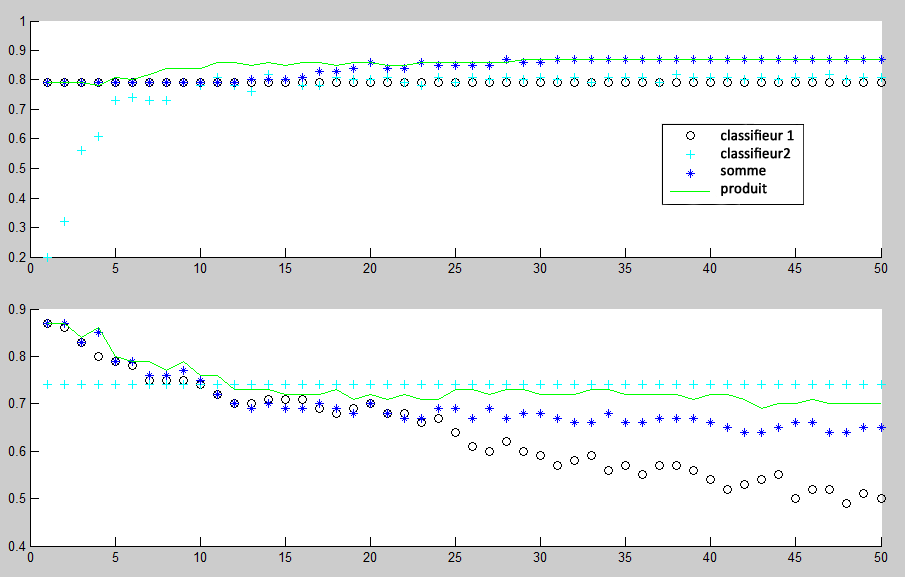
\includegraphics[width=\textwidth]{img/40-rates-function-of-d-k.png}
	\end{center}
	\caption{Variation des quatre taux de reconnaissance obtenus en fonction des paramètres $d$ (en haut) et $k$ (en bas)}
	\label{fig:ratecomparison}
\end{figure}

Globalement on observe de meilleurs résultats pour les combinaisons de classifieurs, représentés dans sur la figure ci-dessus en vert et en bleu foncé. Cependant, si l'on utilise les paramètres optimaux définis précédemment, les résultats sont biaisés : étant donné le paramètre $k$ fixé à 1, les probabilités résultant du second classifieur sont binaire, ce qui annule les résultats du premier classifieur dans le cas du produit mais aussi de la somme.

% CONCLUSION

\end{document}
